\documentclass[12pt,a4paper]{report}

\usepackage[margin=1in]{geometry}
\usepackage[T1]{fontenc}
\usepackage[utf8]{inputenc}
\usepackage{lmodern}
\usepackage{setspace}
\usepackage{hyperref}
\usepackage{longtable}
\usepackage{booktabs}
\usepackage{array}
\usepackage{xcolor}
\usepackage{listings}
\usepackage{enumitem}
\usepackage{tikz}
\usetikzlibrary{arrows.meta,positioning,shapes.geometric}

\hypersetup{
  colorlinks=true,
  linkcolor=blue!45!black,
  urlcolor=blue!55!black,
  citecolor=blue!45!black
}

\definecolor{darkbg}{HTML}{080A0F}
\definecolor{surface}{HTML}{0F1117}
\definecolor{amber}{HTML}{F59E0B}
\definecolor{green}{HTML}{10B981}
\definecolor{blue}{HTML}{3B82F6}
\definecolor{red}{HTML}{EF4444}
\definecolor{muted}{HTML}{64748B}

\lstdefinestyle{codeblock}{
  basicstyle=\ttfamily\small,
  breaklines=true,
  frame=single,
  columns=fullflexible,
  backgroundcolor=\color{gray!6},
  rulecolor=\color{gray!35}
}
\lstset{style=codeblock}

\setstretch{1.18}
\setlist[itemize]{topsep=4pt,itemsep=3pt}
\setlist[enumerate]{topsep=4pt,itemsep=3pt}

\newcommand{\projectname}{Repair Manager}
\newcommand{\stackname}{MERN}

\begin{document}

\begin{titlepage}
  \centering
  \vspace*{1.0cm}
  {\Huge\bfseries \projectname{} Website Report\par}
  \vspace{0.4cm}
  {\Large Full-stack MERN garage repair management system\par}
  \vspace{1.2cm}
  {\large React Frontend \quad Express API \quad MongoDB Database \quad JWT Authentication\par}
  \vfill
  \begin{tabular}{rl}
    Project folder: & \texttt{MERNPROJECT}\\
    Application type: & Full-stack web application\\
    Report date: & April 30, 2026\\
  \end{tabular}
  \vfill
  {\large Prepared as a technical project report and presentation companion\par}
\end{titlepage}

\pagenumbering{roman}
\tableofcontents
\clearpage
\pagenumbering{arabic}

\chapter*{Executive Summary}
\addcontentsline{toc}{chapter}{Executive Summary}

\projectname{} is a full-stack web application built for an auto repair shop or garage. It gives garage staff a secure dashboard for managing customer repair jobs and gives customers a public tracking portal where they can check the status of their vehicle using a tracking code. The website is implemented with the \stackname{} stack: MongoDB for persistence, Express and Node.js for the backend API, and React for the frontend interface.

The application covers the major operational needs of a small repair business: staff authentication, repair job creation, update and deletion, status management, dashboard statistics, cost tracking, search and filtering, and customer-facing status lookup. The backend protects staff routes with JSON Web Tokens (JWTs), scopes repair data to the logged-in user, and exposes a public tracking endpoint that returns only the information needed by customers.

Overall, the project demonstrates a complete and practical CRUD-based business application. Its strongest features are the clear separation between staff and customer workflows, the use of protected API routes, and the repair job tracking code model. Recommended future improvements include automated tests, stronger production secret handling, role-based authorization, input validation hardening, audit history, and cleanup of several frontend text encoding artifacts.

\chapter{Introduction}

\section{Project Background}

Auto repair shops often manage jobs through phone calls, handwritten notes, spreadsheets, or disconnected messaging channels. This can create delays, duplicate records, missing cost information, and weak visibility for both staff and customers. \projectname{} addresses these issues by centralizing repair job management in a web dashboard and exposing a simple tracking interface for customers.

\section{Project Aim}

The aim of the website is to provide a secure, easy-to-use garage management system that supports the complete repair lifecycle from job creation to completion. The application should help staff manage operations and help customers track repairs without requiring a customer account.

\section{Objectives}

The main objectives are:

\begin{itemize}
  \item Provide secure signup and login for garage staff.
  \item Allow authenticated staff to create, view, edit, delete, and complete repair jobs.
  \item Generate stable tracking codes for repair jobs.
  \item Let customers check repair progress from a public tracking page.
  \item Display dashboard statistics such as total jobs, pending jobs, completed jobs, and estimated revenue.
  \item Support search and filtering by status, customer, vehicle, plate, tracking code, and issue description.
  \item Prepare the project for deployment using Vercel for the frontend and Render for the backend.
\end{itemize}

\chapter{Website Overview}

\section{Application Identity}

The website is branded as \projectname{} or \texttt{RepairMGR}. The visual design uses a dark operational dashboard style with amber highlights, status colors, compact panels, and a sidebar navigation system. This design language fits a garage or workshop system because it prioritizes quick scanning, repeated use, and operational clarity.

\section{Target Users}

\begin{longtable}{p{0.24\textwidth}p{0.68\textwidth}}
\toprule
\textbf{User group} & \textbf{Needs supported by the website}\\
\midrule
Garage staff & Secure login, job creation, job updates, status management, cost tracking, dashboard statistics, search, and filtering.\\
Customers & Repair status lookup using a tracking code without logging in.\\
Administrator or owner & Overview of repair workload, completion rate, estimated revenue, and open jobs.\\
\bottomrule
\end{longtable}

\section{Primary Features}

\begin{itemize}
  \item Authentication through signup and login forms.
  \item JWT-protected repair job API.
  \item Repair job CRUD operations.
  \item Repair completion action with completion timestamp.
  \item Customer tracking code lookup.
  \item Dashboard statistics for operational visibility.
  \item Search and status filters.
  \item Responsive frontend layout with a collapsible sidebar.
\end{itemize}

\chapter{Technology Stack}

\section{Frontend}

The frontend is a React application located in \texttt{frontend}. It uses:

\begin{itemize}
  \item \textbf{React 18} for component-based UI.
  \item \textbf{Axios} for API requests.
  \item \textbf{React Scripts} for local development and production builds.
  \item \textbf{Tailwind CSS dependencies} alongside a custom stylesheet in \texttt{src/styles.css}.
  \item Browser \texttt{localStorage} to persist the authenticated staff session.
\end{itemize}

\section{Backend}

The backend is a Node.js and Express API located in \texttt{backend}. It uses:

\begin{itemize}
  \item \textbf{Express} for routing and middleware.
  \item \textbf{Mongoose} for MongoDB models and database access.
  \item \textbf{JSON Web Tokens} for authentication.
  \item \textbf{bcryptjs} for password hashing.
  \item \textbf{cors} for controlled frontend access.
  \item \textbf{dotenv} for environment variables.
\end{itemize}

\section{Database}

MongoDB stores users and repair jobs. The two main collections are:

\begin{itemize}
  \item \texttt{User}: staff account records with name, email, and hashed password.
  \item \texttt{RepairJob}: repair records associated with a user, including tracking code, customer details, car details, issue description, status, costs, and dates.
\end{itemize}

\chapter{System Architecture}

\section{High-Level Architecture}

\begin{center}
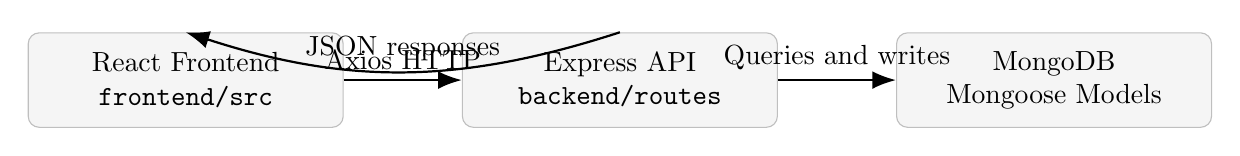
\begin{tikzpicture}[
  node distance=1.5cm,
  box/.style={rectangle, rounded corners, draw=gray!50, fill=gray!8, minimum width=4cm, minimum height=1.2cm, align=center},
  arrow/.style={-{Latex[length=3mm]}, thick}
]
\node[box] (react) {React Frontend\\\texttt{frontend/src}};
\node[box, right=of react] (api) {Express API\\\texttt{backend/routes}};
\node[box, right=of api] (db) {MongoDB\\Mongoose Models};
\draw[arrow] (react) -- node[above]{Axios HTTP} (api);
\draw[arrow] (api) -- node[above]{Queries and writes} (db);
\draw[arrow, bend left=18] (api.north) to node[above]{JSON responses} (react.north);
\end{tikzpicture}
\end{center}

\section{Architecture Explanation}

The React frontend renders the staff dashboard and customer tracking portal. It calls the backend using Axios. Staff requests include a bearer token in the \texttt{Authorization} header. The Express backend validates tokens, applies route protection, and uses Mongoose to read and write MongoDB documents.

The architecture separates public and private workflows:

\begin{itemize}
  \item Public route: customer tracking by repair code.
  \item Private routes: repair job CRUD and staff account information.
\end{itemize}

\section{Folder Structure}

\begin{lstlisting}
MERNPROJECT
|-- README.md
|-- frontend
|   |-- package.json
|   |-- src
|   |   |-- App.jsx
|   |   |-- apiConfig.js
|   |   |-- styles.css
|   |   `-- components
|   |       |-- AuthForm.jsx
|   |       |-- CustomerTrack.jsx
|   |       |-- RepairForm.jsx
|   |       |-- RepairItem.jsx
|   |       `-- RepairList.jsx
`-- backend
    |-- package.json
    |-- server.js
    |-- middleware
    |   `-- authMiddleware.js
    |-- models
    |   |-- RepairJob.js
    |   `-- User.js
    `-- routes
        |-- authRoutes.js
        `-- repairRoutes.js
\end{lstlisting}

\chapter{Frontend Design and Functionality}

\section{Main React Application}

The main frontend component is \texttt{App.jsx}. It manages the application state for authentication, active tabs, repair data, search filters, loading indicators, errors, and sidebar collapse behavior.

Important state values include:

\begin{itemize}
  \item \texttt{user}: current authenticated staff user and JWT token.
  \item \texttt{repairs}: repair jobs fetched from the backend.
  \item \texttt{editingRepair}: selected job being edited.
  \item \texttt{activeTab}: selected dashboard tab.
  \item \texttt{statusFilter} and \texttt{searchTerm}: list filtering controls.
  \item \texttt{publicTrackMode}: switches unauthenticated users into the customer tracking portal.
\end{itemize}

\section{Authentication Interface}

The \texttt{AuthForm.jsx} component supports both login and signup. It renders a branded hero area, authentication fields, and a customer entry action. Staff users submit email and password for login, while signup also requires a full name.

Successful authentication returns a user object and JWT token from the backend. The frontend stores the object in \texttt{localStorage} under \texttt{repairManagerUser}.

\section{Dashboard}

After login, staff users see a dashboard shell with:

\begin{itemize}
  \item Sidebar navigation for Dashboard, All Repairs, New Repair, Completed, and About.
  \item Topbar with breadcrumb and a New Repair action.
  \item Dashboard hero section.
  \item KPI cards for total jobs, pending jobs, in-progress jobs, completed jobs, cancelled jobs, and estimated revenue.
  \item Financial summary and recent repairs.
\end{itemize}

\section{Repair Job Form}

The \texttt{RepairForm.jsx} component handles both job creation and editing. The form captures:

\begin{itemize}
  \item Customer name and phone number.
  \item Car model and license plate.
  \item Issue description.
  \item Status.
  \item Estimated and actual cost.
\end{itemize}

When submitted, numeric cost fields are converted to numbers before they are sent to the API.

\section{Repair List and Repair Cards}

\texttt{RepairList.jsx} renders repair job records by delegating each item to \texttt{RepairItem.jsx}. Each repair card shows customer details, vehicle details, tracking code, costs, status, dates, and days in the garage. Staff users can copy the tracking code, edit the record, delete it, or mark it complete.

\section{Customer Tracking Portal}

\texttt{CustomerTrack.jsx} lets customers enter a tracking code and retrieve public repair information. The portal displays:

\begin{itemize}
  \item Vehicle model.
  \item Tracking code.
  \item Status badge.
  \item Progress steps: Received, In Progress, Completed.
  \item Issue description and basic repair metadata.
\end{itemize}

The tracking portal does not require login, which reduces friction for customers while keeping staff operations protected.

\chapter{Backend Design and Functionality}

\section{Server Setup}

The backend entry point is \texttt{server.js}. It configures:

\begin{itemize}
  \item Express application instance.
  \item JSON body parsing.
  \item CORS origin rules.
  \item Root route and health route.
  \item Authentication routes under \texttt{/api/auth}.
  \item Repair routes under \texttt{/api/repairs}.
  \item 404 handling and error handling middleware.
  \item MongoDB connection through Mongoose.
\end{itemize}

\section{CORS Configuration}

The backend allows local development origin \texttt{http://localhost:3000} and configured deployed frontend URLs. It also includes a helper to allow Vercel preview domains matching the project's expected naming pattern.

\section{Authentication Routes}

\begin{longtable}{p{0.16\textwidth}p{0.32\textwidth}p{0.42\textwidth}}
\toprule
\textbf{Method} & \textbf{Endpoint} & \textbf{Purpose}\\
\midrule
POST & \texttt{/api/auth/signup} & Create a staff user account and return a JWT.\\
POST & \texttt{/api/auth/login} & Validate email/password and return a JWT.\\
GET & \texttt{/api/auth/me} & Return the logged-in staff user's profile.\\
\bottomrule
\end{longtable}

\section{Repair Routes}

\begin{longtable}{p{0.16\textwidth}p{0.36\textwidth}p{0.38\textwidth}}
\toprule
\textbf{Method} & \textbf{Endpoint} & \textbf{Purpose}\\
\midrule
GET & \texttt{/api/repairs/track/:trackingCode} & Public customer lookup by tracking code.\\
POST & \texttt{/api/repairs} & Create a repair job for the logged-in user.\\
GET & \texttt{/api/repairs} & Get repair jobs belonging to the logged-in user.\\
GET & \texttt{/api/repairs/:id} & Get one owned repair job.\\
PUT & \texttt{/api/repairs/:id} & Update one owned repair job.\\
DELETE & \texttt{/api/repairs/:id} & Delete one owned repair job.\\
PATCH & \texttt{/api/repairs/:id/complete} & Mark one owned repair job as completed.\\
\bottomrule
\end{longtable}

\section{Route Protection}

The \texttt{protect} middleware checks for a bearer token, verifies it with the JWT secret, loads the user from MongoDB, and attaches the user to the request object. If validation fails, the backend returns a 401 response.

\chapter{Database Design}

\section{User Model}

The \texttt{User} schema contains:

\begin{itemize}
  \item \texttt{name}: required, trimmed, minimum length 2.
  \item \texttt{email}: required, unique, lowercase, trimmed, and matched against an email pattern.
  \item \texttt{password}: required, minimum length 6, and excluded by default from query results.
  \item timestamps for creation and update dates.
\end{itemize}

Before saving, the schema hashes modified passwords with bcrypt. It also provides a \texttt{matchPassword} method for login verification.

\section{Repair Job Model}

The \texttt{RepairJob} schema contains:

\begin{itemize}
  \item \texttt{user}: owner reference to the staff user.
  \item \texttt{trackingCode}: unique public lookup code.
  \item \texttt{customerName}, \texttt{phoneNumber}, \texttt{carModel}, and \texttt{licensePlate}.
  \item \texttt{issueDescription}: required repair issue details.
  \item \texttt{status}: one of \texttt{pending}, \texttt{in-progress}, \texttt{completed}, or \texttt{cancelled}.
  \item \texttt{estimatedCost} and \texttt{actualCost}.
  \item \texttt{createdAt} and \texttt{completedAt}.
\end{itemize}

\section{Tracking Code Generation}

Tracking codes are generated before validation when no tracking code exists. The code uses the prefix \texttt{RM}, a compact date segment, and a random uppercase alphanumeric segment. This creates codes such as:

\begin{lstlisting}
RM-260430-A1B2C3
\end{lstlisting}

\chapter{User Workflows}

\section{Staff Workflow}

\begin{enumerate}
  \item Staff member creates an account or logs in.
  \item Frontend receives a JWT and stores it in local storage.
  \item Staff member creates a repair job from the New Repair tab.
  \item Backend stores the job and generates a tracking code.
  \item Staff member views, searches, filters, edits, completes, or deletes repair jobs.
  \item Dashboard statistics update after repair data is fetched.
\end{enumerate}

\section{Customer Workflow}

\begin{enumerate}
  \item Customer receives a tracking code from the garage.
  \item Customer opens the tracking portal from the login page.
  \item Customer enters the tracking code.
  \item Frontend calls the public tracking endpoint.
  \item Customer sees vehicle status, issue description, costs, and dates.
\end{enumerate}

\chapter{Security Analysis}

\section{Current Security Strengths}

\begin{itemize}
  \item Passwords are hashed with bcrypt before storage.
  \item Staff routes are protected with JWT authentication.
  \item Repair jobs are scoped to the logged-in user.
  \item Tracking codes are stable and separate from database IDs.
  \item Public tracking endpoint returns limited fields rather than the full internal record.
  \item CORS rules restrict browser access to expected frontend origins.
\end{itemize}

\section{Security Improvements}

\begin{itemize}
  \item Require a strong production \texttt{JWT\_SECRET}; avoid using the development fallback in production.
  \item Add server-side validation with a library such as Zod, Joi, or express-validator.
  \item Add rate limiting to authentication and tracking endpoints.
  \item Add role-based authorization if the system grows beyond one staff role.
  \item Store JWTs in secure HTTP-only cookies for stronger browser-side protection.
  \item Add audit logs for deletion and completion actions.
\end{itemize}

\chapter{Deployment}

\section{Frontend Deployment}

The README describes Vercel deployment for the frontend:

\begin{lstlisting}
Root Directory: frontend
Build Command: npm run build
Output Directory: build
\end{lstlisting}

The frontend uses \texttt{REACT\_APP\_API\_URL} to point to the deployed backend API.

\section{Backend Deployment}

The README describes Render deployment for the backend:

\begin{lstlisting}
Root Directory: backend
Build Command: npm install
Start Command: npm start
\end{lstlisting}

Required backend environment variables include:

\begin{itemize}
  \item \texttt{PORT}
  \item \texttt{MONGO\_URI}
  \item \texttt{JWT\_SECRET}
  \item \texttt{CLIENT\_URLS}
\end{itemize}

\section{Database Deployment}

For production, MongoDB Atlas can be used as the hosted database provider. The backend should be configured with a MongoDB connection string in \texttt{MONGO\_URI}. Network access should be restricted appropriately for production rather than left open broadly.

\chapter{Testing and Quality}

\section{Suggested Test Plan}

\begin{longtable}{p{0.24\textwidth}p{0.66\textwidth}}
\toprule
\textbf{Test area} & \textbf{Recommended checks}\\
\midrule
Authentication & Signup, duplicate email rejection, login success, login failure, token expiry behavior.\\
Repair CRUD & Create, list, edit, delete, and complete repair jobs.\\
Authorization & Confirm users cannot access another user's repair jobs.\\
Tracking portal & Valid tracking code, invalid tracking code, public response field limits.\\
Dashboard & KPI totals, completion rate, estimated revenue, actual revenue, average cost.\\
Search/filter & Search by customer, car, plate, issue, and tracking code; filter by each status.\\
Responsive UI & Desktop, tablet, and mobile layouts.\\
Deployment & Vercel frontend environment, Render backend environment, MongoDB Atlas connectivity.\\
\bottomrule
\end{longtable}

\section{Current Quality Observations}

\begin{itemize}
  \item The codebase is organized clearly around frontend and backend responsibilities.
  \item The API routes are readable and aligned with the user workflows.
  \item The frontend dashboard is feature-rich for a small business application.
  \item The source includes several text encoding artifacts around arrows, dashes, and icon text; these should be cleaned before final submission or production use.
  \item No automated test files are present in the repository at the time of this report.
\end{itemize}

\chapter{Limitations}

The current version is a strong functional prototype, but it has limitations:

\begin{itemize}
  \item It uses one staff role and does not yet support different permissions.
  \item Repair history is represented by the current record rather than a detailed status timeline.
  \item Public tracking exposes cost fields, which may or may not be desirable depending on business policy.
  \item There is no file upload for invoices, photos, or inspection reports.
  \item There are no automated unit, integration, or end-to-end tests in the repository.
  \item Frontend images are loaded from external URLs, which may fail if network access is unavailable.
\end{itemize}

\chapter{Future Enhancements}

Recommended future enhancements include:

\begin{itemize}
  \item Add role-based access control for owner, manager, and mechanic roles.
  \item Add a repair status timeline with notes and timestamps.
  \item Add customer notifications by email or SMS.
  \item Add invoice generation and printable job cards.
  \item Add photo uploads for vehicle condition and repair evidence.
  \item Add analytics for revenue, completion time, common issues, and mechanic workload.
  \item Add automated tests for API routes and core React workflows.
  \item Add stronger validation and rate limiting on public endpoints.
  \item Add dark/light theme preference if needed by staff users.
\end{itemize}

\chapter{Conclusion}

\projectname{} successfully demonstrates a complete MERN website for garage repair management. It combines secure staff authentication, repair job lifecycle management, dashboard reporting, and public customer tracking in a coherent full-stack architecture. The project is practical, easy to understand, and ready for further hardening through tests, validation, role management, and production security improvements.

The website is especially effective as a student or portfolio project because it shows both user-facing design and backend engineering: React state management, REST API design, JWT authentication, database schemas, protected routes, deployment configuration, and business workflow modeling.

\appendix
\chapter{Key Files Reviewed}

\begin{itemize}
  \item \texttt{README.md}
  \item \texttt{frontend/package.json}
  \item \texttt{frontend/src/App.jsx}
  \item \texttt{frontend/src/apiConfig.js}
  \item \texttt{frontend/src/styles.css}
  \item \texttt{frontend/src/components/AuthForm.jsx}
  \item \texttt{frontend/src/components/CustomerTrack.jsx}
  \item \texttt{frontend/src/components/RepairForm.jsx}
  \item \texttt{frontend/src/components/RepairItem.jsx}
  \item \texttt{frontend/src/components/RepairList.jsx}
  \item \texttt{backend/server.js}
  \item \texttt{backend/models/User.js}
  \item \texttt{backend/models/RepairJob.js}
  \item \texttt{backend/routes/authRoutes.js}
  \item \texttt{backend/routes/repairRoutes.js}
  \item \texttt{backend/middleware/authMiddleware.js}
\end{itemize}

\chapter{Local Run Commands}

\section{Backend}
\begin{lstlisting}
cd backend
npm install
npm run dev
\end{lstlisting}

\section{Frontend}
\begin{lstlisting}
cd frontend
npm install --legacy-peer-deps
npm start
\end{lstlisting}

\section{Production Build}
\begin{lstlisting}
cd frontend
npm run build
\end{lstlisting}

\end{document}
